%%%%%%%%%%%%%%%%%%%%%%%%%%%%%%%%%%%%%%%%%%%%%%%%%%%%%%%%%%%%%%%%%%%%%%%%%%%%%%%
% Chapter 'Absorption - R-134a - TriEGDME '
%%%%%%%%%%%%%%%%%%%%%%%%%%%%%%%%%%%%%%%%%%%%%%%%%%%%%%%%%%%%%%%%%%%%%%%%%%%%%%%
\subsection{Triegdme }
%
%%%%%%%%%%%%%%%%%%%%%%%%%%%%%%%%%%%%%%%%%%%%%%%%%%%%%%%%%%%%%%%%%%%%%%%%%%%%%%%
%%%%%%%%%%%%%%%%%%%%%%%%%%%%%%%%%%%%%%%%%%%%%%%%%%%%%%%%%%%%%%%%%%%%%%%%%%%%%%%
\subsubsection{WilsonTemperatureDl - ID 1}
%
\begin{tabular}[l]{|lp{11.5cm}|}
\hline
\addlinespace

\textbf{Sorbent:} & TriEGDME \\
\textbf{Subtype:} &  \\
\textbf{Refrigerant:} & R-134a \\
\textbf{Equation:} & WilsonTemperatureDl \\
\textbf{ID:} & 1 \\
\textbf{Reference:} & Marchi, Paolo; Scalabrin, Giancarlo; Ihmels, E. Christian; Fischer, Kai; Gmehling, Jürgen (2006): Bubble pressure measurements for the (1,1,1,2-tetrafluoroethane+triethylene glycol dimethyl ether) system. In: The Journal of Chemical Thermodynamics 38 (11), S. 1247–1253. DOI: 10.1016/j.jct.2006.03.004. \\
\textbf{Comment:} & See original literature: Use low-level interface to input molar volumes of both components, which are calculated by propper equations of state (i.e., v\_POE =   1/((61.387-0.024138*((T-273.15)*1.8+32))*16.0185)*0.59 in m3/mol), for calculations. \\

\addlinespace
\hline
\end{tabular}
\newline

\textbf{Equation and parameters:}
\newline
%
Pressure $p$ in $\si{\pascal}$ is calculated depending on molar fraction of refrigerant in the liquid phase $x_1$ in $\si{\mole\per\mole}$, temperature $T$ in $\si{\kelvin}$, molar volumes of both components ($v_1$ and $v_2$) in $\si{\cubic\meter\per\mole}$, and vapor pressure $p_\mathrm{sat,1}$ in $\si{\pascal}$. If molar volumes less than zero are used as function arguements, constant molar volumes given by parameter record are used. Equilibrium equation is given by:
%
\begin{equation*}
\begin{split}
p &=& \gamma_1 x_1 p_\mathrm{sat,1} & \quad\text{, and} \\
\gamma_1 &=& \exp \left( - \ln \left( x_1 + \Lambda_{12} x_2 \right) + x_2 \left( \frac{\Lambda_{12}}{x_1 + \Lambda_{12} x_2} - \frac{\Lambda_{21}}{x_2 + \Lambda_{21} x_1} \right) \right) & \quad\text{, and} \\
\Lambda_{12} &=& \nicefrac{v_2}{v_1} \exp \left( - \frac{\Delta\lambda_{12}}{R T} \right) & \quad\text{, and} \\
\Lambda_{21} &=& \nicefrac{v_1}{v_2} \exp \left( - \frac{\Delta\lambda_{21}}{R T} \right) & \quad\text{, and} \\
\Delta\lambda_{12} &=& R \left( \Delta\lambda_\mathrm{12,c} + \Delta\lambda_\mathrm{12,t} \left( T - c \right) \right) & \quad\text{, and} \\
\Delta\lambda_{21} &=& R \left( \Delta\lambda_\mathrm{21,c} + \Delta\lambda_\mathrm{21,t} \left( T - c \right) \right) & \quad\text{, and} \\
x_2 &=& 1 - x_1  & \quad\text{.} \\
\end{split}
\end{equation*}
%
The parameters of the equation are:
%
\begin{longtable}[l]{lll|lll}
\toprule
\addlinespace
\textbf{Par.} & \textbf{Unit} & \textbf{Value} &	\textbf{Par.} & \textbf{Unit} & \textbf{Value} \\
\addlinespace
\midrule
\endhead

\bottomrule
\endfoot
\bottomrule
\endlastfoot
\addlinespace

$\Delta\lambda_\mathrm{12,c}$ & $\si{\kelvin}$ & -1.491280000e+02 & $\Delta\lambda_\mathrm{21,c}$ & $\si{\kelvin}$ & 3.681890000e+02 \\
$\Delta\lambda_\mathrm{12,t}$ & - & 9.592910000e-01 & $\Delta\lambda_\mathrm{12,t}$ & - & 9.291260000e-01 \\
$v_1$ & $\si{\cubic\meter\per\mole}$ & 1.000000000e+00 & $v_2$ & $\si{\cubic\meter\per\mole}$ & 1.000000000e+00 \\
$c$ & $\si{\kelvin}$ & 2.731500000e+02 & & & \\

\addlinespace\end{longtable}

\textbf{Validity:}
\newline
Equation is approximately valid for $283.15 \si{\kelvin} \leq T \leq 323.15 \si{\kelvin}$.
\newline

\textbf{Visualization:}
%
\begin{figure}[!htp]
{\noindent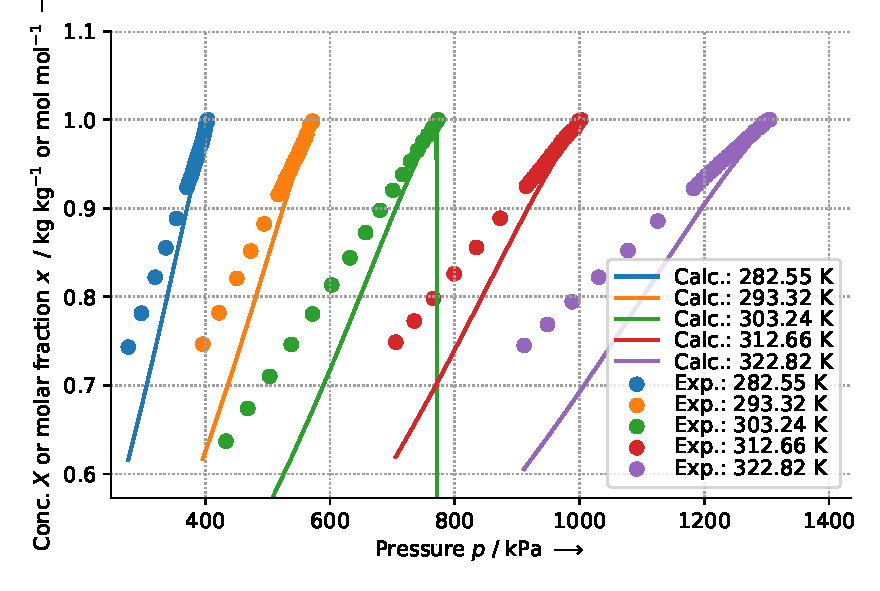
\includegraphics[height=10cm, keepaspectratio]{figs/abs/abs_R-134a_TriEGDME__WilsonTemperatureDl_1.pdf}}
\end{figure}
%

To generate the figure, the following refrigerant functions were selected:
\begin{itemize}
\item Vapor pressure: VaporPressure\_EoS1 - ID 1
\item Saturated liquid density: SaturatedLiquidDensity\_EoS1 - ID 1
\item Special refrigerant functions as described by comment and CoolProp
\end{itemize}

The uncertainity of the experimental data is:
\begin{itemize}
\item Data source $\,\to\,$ Data was taken from table
\item Pressure, absolute, in $\si{\pascal}$ $\,\to\,$ 1.00E+02
\item Temperature, absolute, in $\si{\kelvin}$ $\,\to\,$ 0.03
\end{itemize}

The mean absolute percentage error (MAPE) between the experimental and calculated data results in 5.69\%.
\FloatBarrier
\newpage
%%%%%%%%%%%%%%%%%%%%%%%%%%%%%%%%%%%%%%%%%%%%%%%%%%%%%%%%%%%%%%%%%%%%%%%%%%%%%%%
